\setcounter{figure}{0}

\section{17th September 2023: Words of affirmation}
\subsection*{Text: Song of Solomon 6:4-7:10}
  \begin{quote}
    He

    [4] You are beautiful as Tirzah, my love,
        lovely as Jerusalem,
        awesome as an army with banners.
    [5] Turn away your eyes from me,
        for they overwhelm me—
    Your hair is like a flock of goats
        leaping down the slopes of Gilead.
    [6] Your teeth are like a flock of ewes
        that have come up from the washing;
    all of them bear twins;
        not one among them has lost its young.
    [7] Your cheeks are like halves of a pomegranate
        behind your veil.
    [8] There are sixty queens and eighty concubines,
        and virgins without number.
    [9] My dove, my perfect one, is the only one,
        the only one of her mother,
        pure to her who bore her.
    The young women saw her and called her blessed;
        the queens and concubines also, and they praised her.


    [10] “Who is this who looks down like the dawn,
        beautiful as the moon, bright as the sun,
        awesome as an army with banners?”


    She

    [11] I went down to the nut orchard
        to look at the blossoms of the valley,
    to see whether the vines had budded,
        whether the pomegranates were in bloom.
    [12] Before I was aware, my desire set me
        among the chariots of my kinsman, a prince.


    Others

    [13] Return, return, O Shulammite,
        return, return, that we may look upon you.


    He

    Why should you look upon the Shulammite,
        as upon a dance before two armies?


    [1] How beautiful are your feet in sandals,
        O noble daughter!
    Your rounded thighs are like jewels,
        the work of a master hand.
    [2] Your navel is a rounded bowl
        that never lacks mixed wine.
    Your belly is a heap of wheat,
        encircled with lilies.
    [3] Your two breasts are like two fawns,
        twins of a gazelle.
    [4] Your neck is like an ivory tower.
    Your eyes are pools in Heshbon,
        by the gate of Bath-rabbim.
    Your nose is like a tower of Lebanon,
        which looks toward Damascus.
    [5] Your head crowns you like Carmel,
        and your flowing locks are like purple;
        a king is held captive in the tresses.


    [6] How beautiful and pleasant you are,
        O loved one, with all your delights!
    [7] Your stature is like a palm tree,
        and your breasts are like its clusters.
    [8] I say I will climb the palm tree
        and lay hold of its fruit.
    Oh may your breasts be like clusters of the vine,
        and the scent of your breath like apples,
    [9] and your mouth like the best wine.


    She

    It goes down smoothly for my beloved,
        gliding over lips and teeth.


    [10] I am my beloved’s,
        and his desire is for me.
  \end{quote}
\subsection*{Notes}
\begin{itemize}
  \item{To think: why do couples treat each other differently before and after marriage?}
  \item{Marriage is not the end of a r/s, it is the start of a lifelong pursuit.}
  \item{In today’s text, the man is always telling the woman how beautiful she is. He has been doing this since their courtship says, and he did this during the wedding, and he is doing it now after marriage again. He is also doing it after a fight (c.f 6:4, 7:1,6).}
  \item{Btw, today’s text is q similar to chapter 4:1-3, very similar metaphors are used.}
  \item{Seems like today’s text show that the man and woman have reconciled after their fight (see ch6:12, ch7:10). No doubt these words of love were helpful; they show the other person that regardless of how bad the fight is, the affection that y’all have for each other is unchanged, and hence they provide the security for the other person to be vulnerable. }
  \item{And ofc, the same principle holds for other interpersonal r/s too (maybe without the erotic component). In our friendships/dealing with our families, we must still love the other person and demonstrate our love even in the midst of a conflict. This demonstration would look like a desire for reconciliation, a seeking for the other person’s forgiveness, a seeking to make restitution for the wrong inflicted, etc. And when we do so, the other person will feel safe to be vulnerable with us and let us know how exactly we hurt them, and then when we address the hurt, this would lead to a growth in closeness and finally reconciliation.}
  \item{In our text, in v4, tirzah and jerusalem are the two capital cities of israel and judah back then. And then there’s also the phrase “awesome as an army with banners”. The same phrase appears in v10, that’s how we know its an inclusio. The whole chunk here then is a description of the wife’s beauty. In this section, the focus is on the wife’s face.}
  \item{The next chunk here in the description of the woman’s beauty is in ch6:13-7:5. The description here starts from bottom up. Some metaphors to take note: damascus is the capital city of the syrians, which are israel’s enemies. Hence the woman’s nose pointing towards damascus signifies an unfearing and brave spirit (much like what is praised in 1 peter 3:1-7). }
  \item{The tl;dr is then this: the woman is beautiful.}
  \item{Here, we also see that the man here is a one-woman man (chapter 6:v9). Unlike solomon!!!!}
  \item{A note on the theology of the body:
  \begin{itemize}
    \item{Bodily beauty points to the beauty of the creator. In fact, all beauty points toward the beauty of God. All creation praises God, and they do so by radiating their beauty, through which we see the wisdom and the beauty of God. Humans best reflect God’s beauty, since is humans are made in the image of God. The image of God should point us back to God.}
    \item{Jesus’ incarnation, death and resurrection took place while He was in the body. God cares about the body! In the future, there will be a \textbf{bodily resurrection}!}
  \end{itemize}}
  \item{Application: husband and wife should continue appreciating each other, physical beauty included! And when we do this, we will see God :).}
  \item{Application 2: we also shouldn’t need to chase after an ideal body image, because that differs from culture to culture! In the past, people loved women with pudgy bodies (e.g belly like a heap of wheat). Defo not today. Each of us has been fearfully and wonderfully made by God, so we should be thankful for the physical qualities God has given us :). In fact, appreciation of physical appearance is in the eye of the beholder! Shulammite thinks she is dark, but the man loves her for it.}
  \item{Application 3: in fact when we look at the man’s description of his wife, not all his description are of the wife’s physical appearance, some of them are of the wife’s qualities. E.g, nose like the tower of lebanon that looks towards damascus-> confidence. Awesome as an army with banners -> exudes strength. }
  % \item{\begin{figure}[H]
  %   \centering
  %   % 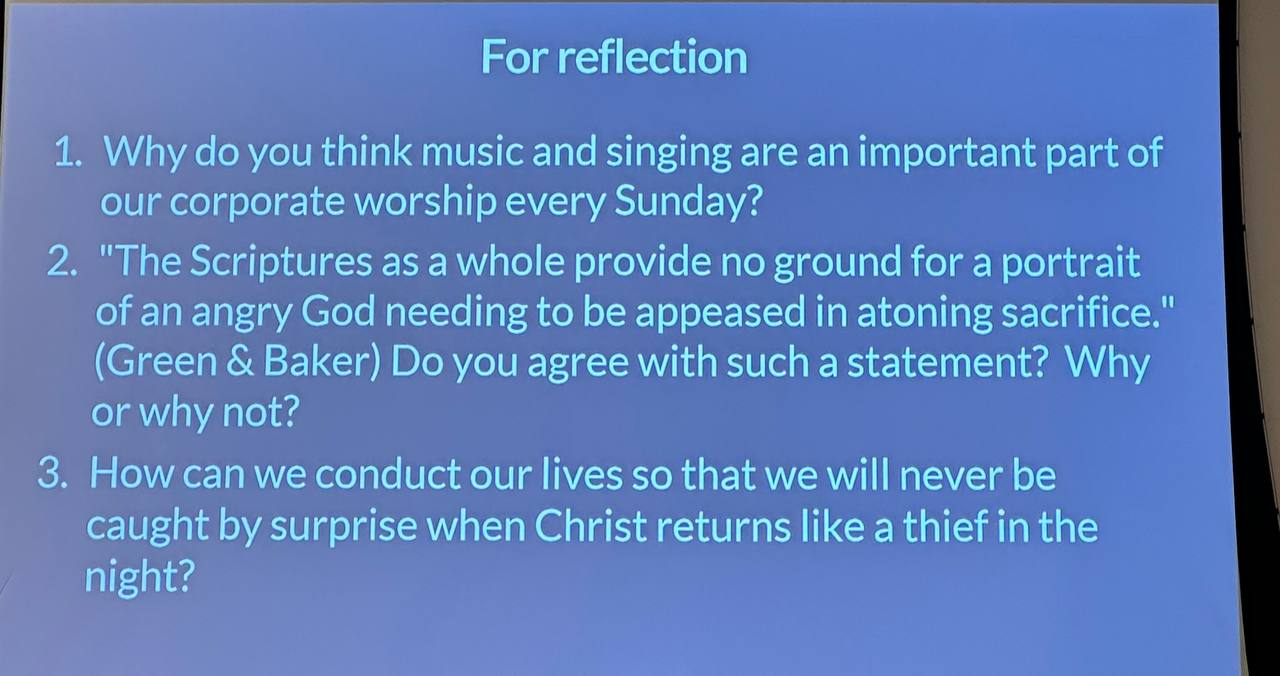
\includegraphics[width=0.8\textwidth, trim={0cm 0cm 0cm 0cm},clip]{Figures/marchSermon4Reflections.jpg}
  %   \includegraphics[width=0.8\textwidth, trim={0cm 0cm 0cm 0cm},clip]{example-image-a}
  %   \caption[]{Reflection questions for this sermon}
  %   \label{}
  % \end{figure}}
\end{itemize}